\documentclass{article}
\usepackage{tikz}
\usetikzlibrary{calc}
%code adapted by Alex Albright from https://sites.google.com/site/kochiuyu/Tikz#TOC-Signalling-Game
%Thank you Chiu Yu Ko (高超禹)!

\begin{document}

\begin{figure}[h]
\centering
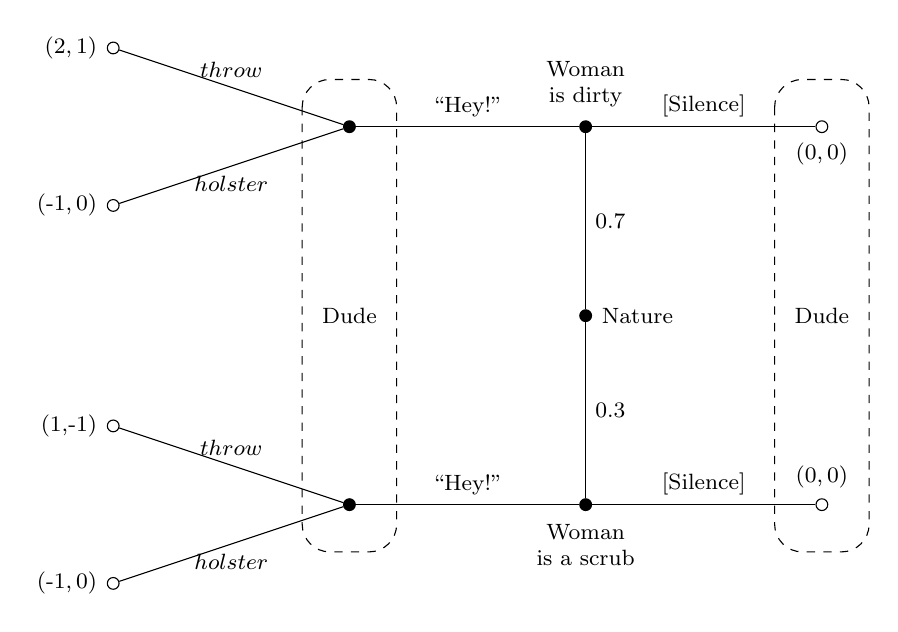
\begin{tikzpicture}[scale=2,font=\footnotesize]
\tikzset{
% Two node styles for game trees: solid and hollow
solid node/.style={circle,draw,inner sep=1.5,fill=black},
hollow node/.style={circle,draw,inner sep=1.5}
}

% Specify spacing for each level of the tree
\tikzstyle{level 1}=[level distance=12mm,sibling distance=25mm]
\tikzstyle{level 2}=[level distance=15mm,sibling distance=15mm]
\tikzstyle{level 3}=[level distance=15mm,sibling distance=10mm]
% The Tree
\node(0)[solid node,label=right:{Nature}]{}
child[grow=up]{node[solid node,label=above:{\begin{tabular}{c}
Woman\\ is dirty
\end{tabular}}] {}
child[grow=left]{node(1)[solid node]{}
child{node[hollow node,label=left:{$(2,1)$}]{} edge from parent node [above]{$throw$}}
child{node[hollow node,label=left:{$($-1$,0)$}]{} edge from parent node [below]{$holster$}}
edge from parent node [above]{``Hey!"}
}
child[grow=right]{node(3)[hollow node, label=below:{$(0,0)$}]{}
edge from parent node [above]{[Silence]}
}
edge from parent node [right]{$0.7$}
}
child[grow=down]{node[solid node,label=below:{\begin{tabular}{c}
Woman\\ is a scrub
\end{tabular}}] {}
child[grow=left]{node(2)[solid node]{}
child{node[hollow node,label=left:{$(1,$-1$)$}]{} edge from parent node [above]{$throw$}}
child{node[hollow node,label=left:{$($-1$,0)$}]{} edge from parent node [below]{$holster$}}
edge from parent node [above]{``Hey!"}
}
child[grow=right]{node(4)[hollow node, label=above:{$(0,0)$}]{}
edge from parent node [above]{[Silence]}
}
edge from parent node [right]{$0.3$}
};

% information set
\draw[dashed,rounded corners=10]($(1) + (-.3,.3)$)rectangle($(2) +(.3,-.3)$);
\draw[dashed,rounded corners=10]($(3) + (-.3,.3)$)rectangle($(4) +(.3,-.3)$);
% specify mover at 2nd information set
\node at ($(1)!.5!(2)$) {Dude};
\node at ($(3)!.5!(4)$) {Dude};
\end{tikzpicture}


\caption{The ``throw it to the girl" Game in Extensive Form} \label{fig:M1}
\end{figure}

\begin{figure}[h]
\centering
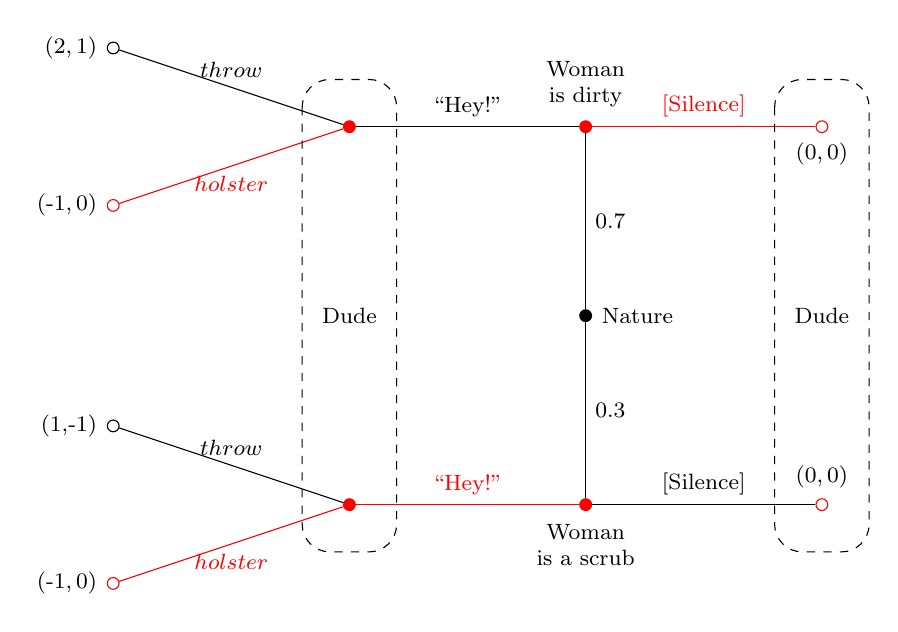
\begin{tikzpicture}[scale=2,font=\footnotesize]
\tikzset{
% Two node styles for game trees: solid and hollow
solid node/.style={circle,draw,inner sep=1.5,fill=black},
hollow node/.style={circle,draw,inner sep=1.5},
emph/.style={edge from parent/.style={red,draw}},
nah/.style={edge from parent/.style={black,draw}}
}

% Specify spacing for each level of the tree
\tikzstyle{level 1}=[level distance=12mm,sibling distance=25mm]
\tikzstyle{level 2}=[level distance=15mm,sibling distance=15mm]
\tikzstyle{level 3}=[level distance=15mm,sibling distance=10mm]
% The Tree
\node(0)[solid node,label=right:{Nature}]{}
child[grow=up]{node[solid node,style={red},label=above:{\begin{tabular}{c}
Woman\\ is dirty
\end{tabular}}] {}
child[grow=left]{node(1)[solid node, style={red}]{}
child{node[hollow node,label=left:{$(2,1)$}]{} edge from parent node [above]{$throw$}}
child[emph]{node[style={red},hollow node,label=left:{$($-1$,0)$}]{} edge from parent node [below]{$holster$}}
edge from parent node [above]{``Hey!"}
}
child[emph, grow=right]{node(3)[hollow node, style={red}, label=below:{$(0,0)$}]{}
edge from parent node [above]{[Silence]}
}
edge from parent node [right]{$0.7$}
}
child[grow=down]{node[solid node, style={red},label=below:{\begin{tabular}{c}
Woman\\ is a scrub
\end{tabular}}] {}
child[emph, grow=left]{node(2)[solid node, style={red}]{}
child[nah]{node[hollow node, style={black}, label=left:{$(1,$-1$)$}]{} edge from parent node [above]{$throw$}}
child{node[hollow node, label=left:{$($-1$,0)$}]{} edge from parent node [below]{$holster$}}
edge from parent node [above]{``Hey!"}
}
child[grow=right]{node(4)[hollow node, style={red}, label=above:{$(0,0)$}]{}
edge from parent node [above]{[Silence]}
}
edge from parent node [right]{$0.3$}
};

% information set
\draw[dashed,rounded corners=10]($(1) + (-.3,.3)$)rectangle($(2) +(.3,-.3)$);
\draw[dashed,rounded corners=10]($(3) + (-.3,.3)$)rectangle($(4) +(.3,-.3)$);
% specify mover at 2nd information set
\node at ($(1)!.5!(2)$) {Dude};
\node at ($(3)!.5!(4)$) {Dude};
\end{tikzpicture}


\caption{Dirty is silent \& Scrub calls} \label{fig:M1}
\end{figure}


\begin{figure}[h]
\centering
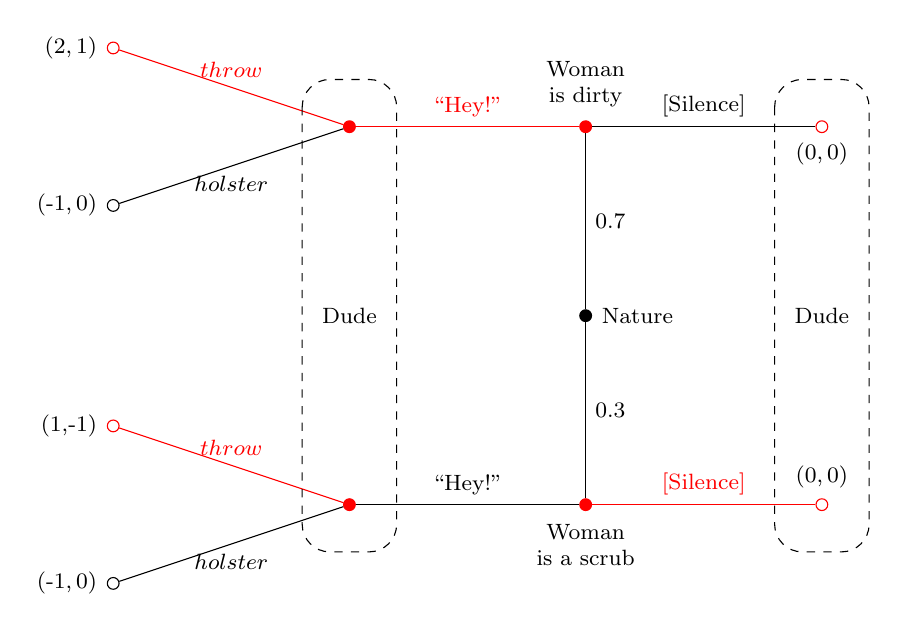
\begin{tikzpicture}[scale=2,font=\footnotesize]
\tikzset{
% Two node styles for game trees: solid and hollow
solid node/.style={circle,draw,inner sep=1.5,fill=black},
hollow node/.style={circle,draw,inner sep=1.5},
emph/.style={edge from parent/.style={red,draw}},
nah/.style={edge from parent/.style={black,draw}}
}

% Specify spacing for each level of the tree
\tikzstyle{level 1}=[level distance=12mm,sibling distance=25mm]
\tikzstyle{level 2}=[level distance=15mm,sibling distance=15mm]
\tikzstyle{level 3}=[level distance=15mm,sibling distance=10mm]
% The Tree
\node(0)[solid node,label=right:{Nature}]{}
child[grow=up]{node[solid node, style={red},label=above:{\begin{tabular}{c}
Woman\\ is dirty
\end{tabular}}] {}
child[grow=left, emph]{node(1)[solid node, style={red}]{}
child{node[hollow node,label=left:{$(2,1)$}]{} edge from parent node [above]{$throw$}}
child[nah]{node[hollow node,style={black},label=left:{$($-1$,0)$}]{} edge from parent node [below]{$holster$}}
edge from parent node [above]{``Hey!"}
}
child[grow=right]{node(3)[hollow node, style={red}, label=below:{$(0,0)$}]{}
edge from parent node [above]{[Silence]}
}
edge from parent node [right]{$0.7$}
}
child[grow=down]{node[solid node,style={red},label=below:{\begin{tabular}{c}
Woman\\ is a scrub
\end{tabular}}] {}
child[grow=left]{node(2)[solid node, style={red}]{}
child[emph]{node[hollow node, style={red},label=left:{$(1,$-1$)$}]{} edge from parent node [above]{$throw$}}
child{node[hollow node,label=left:{$($-1$,0)$}]{} edge from parent node [below]{$holster$}}
edge from parent node [above]{``Hey!"}
}
child[grow=right, emph]{node(4)[hollow node, style={red}, label=above:{$(0,0)$}]{}
edge from parent node [above]{[Silence]}
}
edge from parent node [right]{$0.3$}
};

% information set
\draw[dashed,rounded corners=10]($(1) + (-.3,.3)$)rectangle($(2) +(.3,-.3)$);
\draw[dashed,rounded corners=10]($(3) + (-.3,.3)$)rectangle($(4) +(.3,-.3)$);
% specify mover at 2nd information set
\node at ($(1)!.5!(2)$) {Dude};
\node at ($(3)!.5!(4)$) {Dude};
\end{tikzpicture}


\caption{Dirty calls \& Scrub is silent} \label{fig:M1}
\end{figure}


\begin{figure}[h]
\centering
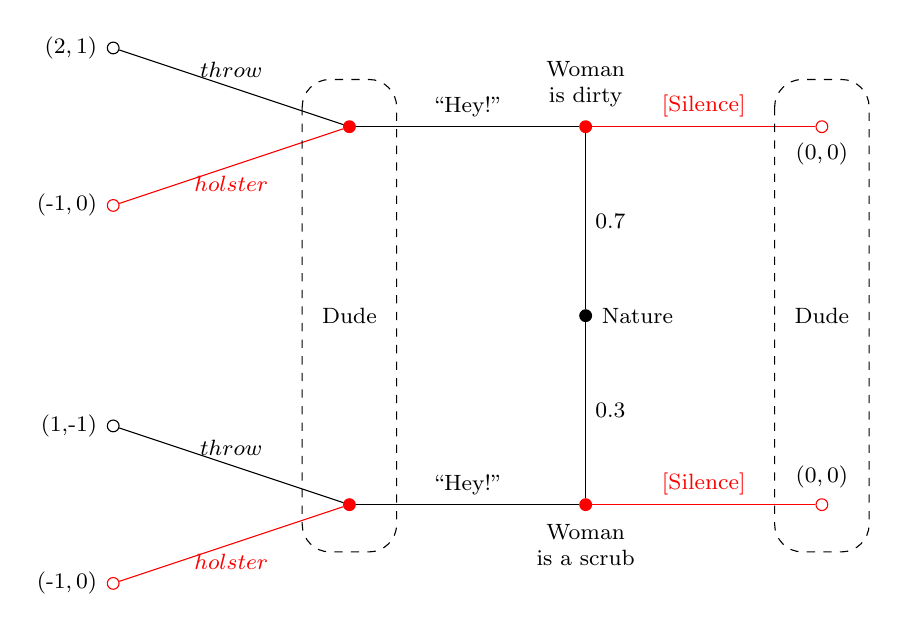
\begin{tikzpicture}[scale=2,font=\footnotesize]
\tikzset{
% Two node styles for game trees: solid and hollow
solid node/.style={circle,draw,inner sep=1.5,fill=black},
hollow node/.style={circle,draw,inner sep=1.5},
emph/.style={edge from parent/.style={red,draw}},
nah/.style={edge from parent/.style={black,draw}}
}

% Specify spacing for each level of the tree
\tikzstyle{level 1}=[level distance=12mm,sibling distance=25mm]
\tikzstyle{level 2}=[level distance=15mm,sibling distance=15mm]
\tikzstyle{level 3}=[level distance=15mm,sibling distance=10mm]
% The Tree
\node(0)[solid node,label=right:{Nature}]{}
child[grow=up]{node[solid node, style={red},label=above:{\begin{tabular}{c}
Woman\\ is dirty
\end{tabular}}] {}
child[grow=left]{node(1)[solid node, style={red}]{}
child{node[hollow node,label=left:{$(2,1)$}]{} edge from parent node [above]{$throw$}}
child[emph]{node[hollow node,style={red},label=left:{$($-1$,0)$}]{} edge from parent node [below]{$holster$}}
edge from parent node [above]{``Hey!"}
}
child[grow=right, emph]{node(3)[hollow node, style={red}, label=below:{$(0,0)$}]{}
edge from parent node [above]{[Silence]}
}
edge from parent node [right]{$0.7$}
}
child[grow=down]{node[solid node, style={red}, label=below:{\begin{tabular}{c}
Woman\\ is a scrub
\end{tabular}}] {}
child[grow=left]{node(2)[solid node, style={red}]{}
child{node[hollow node,label=left:{$(1,$-1$)$}]{} edge from parent node [above]{$throw$}}
child[emph]{node[hollow node,style={red},label=left:{$($-1$,0)$}]{} edge from parent node [below]{$holster$}}
edge from parent node [above]{``Hey!"}
}
child[grow=right, emph]{node(4)[hollow node, style={red}, label=above:{$(0,0)$}]{}
edge from parent node [above]{[Silence]}
}
edge from parent node [right]{$0.3$}
};

% information set
\draw[dashed,rounded corners=10]($(1) + (-.3,.3)$)rectangle($(2) +(.3,-.3)$);
\draw[dashed,rounded corners=10]($(3) + (-.3,.3)$)rectangle($(4) +(.3,-.3)$);
% specify mover at 2nd information set
\node at ($(1)!.5!(2)$) {Dude};
\node at ($(3)!.5!(4)$) {Dude};
\end{tikzpicture}


\caption{Dirty is silent \& Scrub is silent} \label{fig:M1}
\end{figure}

\begin{figure}[h]
\centering
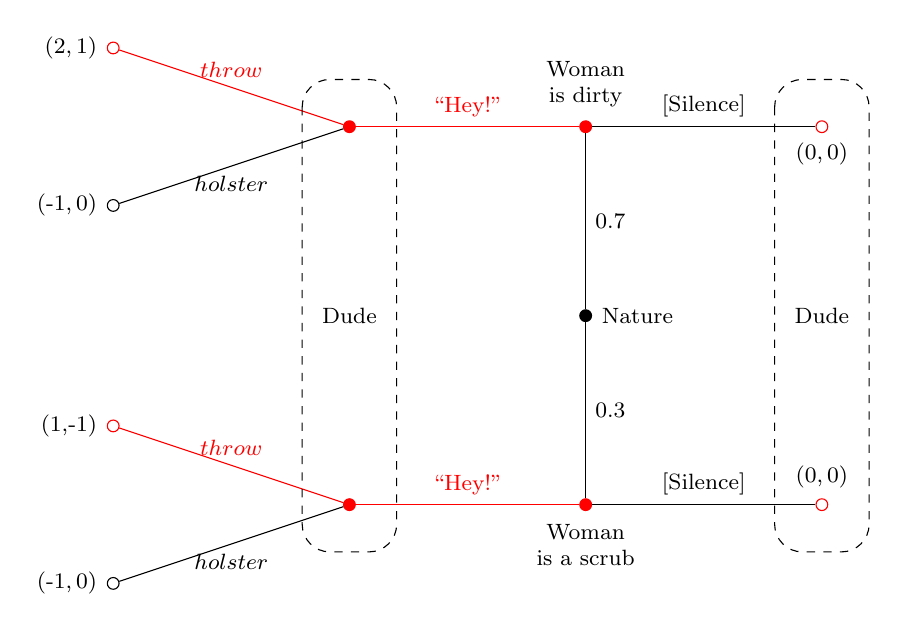
\begin{tikzpicture}[scale=2,font=\footnotesize]
\tikzset{
% Two node styles for game trees: solid and hollow
solid node/.style={circle,draw,inner sep=1.5,fill=black},
hollow node/.style={circle,draw,inner sep=1.5},
emph/.style={edge from parent/.style={red,draw}},
nah/.style={edge from parent/.style={black,draw}}
}

% Specify spacing for each level of the tree
\tikzstyle{level 1}=[level distance=12mm,sibling distance=25mm]
\tikzstyle{level 2}=[level distance=15mm,sibling distance=15mm]
\tikzstyle{level 3}=[level distance=15mm,sibling distance=10mm]
% The Tree
\node(0)[solid node,label=right:{Nature}]{}
child[grow=up]{node[solid node, style={red},label=above:{\begin{tabular}{c}
Woman\\ is dirty
\end{tabular}}] {}
child[emph, grow=left]{node(1)[solid node, style={red}]{}
child{node[hollow node,label=left:{$(2,1)$}]{} edge from parent node [above]{$throw$}}
child[nah] {node[hollow node, style={black},label=left:{$($-1$,0)$}]{} edge from parent node [below]{$holster$}}
edge from parent node [above]{``Hey!"}
}
child[grow=right]{node(3)[hollow node, style={red},label=below:{$(0,0)$}]{}
edge from parent node [above]{[Silence]}
}
edge from parent node [right]{$0.7$}
}
child[grow=down]{node[solid node, style={red},label=below:{\begin{tabular}{c}
Woman\\ is a scrub
\end{tabular}}] {}
child[emph, grow=left]{node(2)[solid node, style={red}]{}
child{node[hollow node,label=left:{$(1,$-1$)$}]{} edge from parent node [above]{$throw$}}
child[nah]{node[hollow node,style={black},label=left:{$($-1$,0)$}]{} edge from parent node [below]{$holster$}}
edge from parent node [above]{``Hey!"}
}
child[grow=right]{node(4)[hollow node, style={red}, label=above:{$(0,0)$}]{}
edge from parent node [above]{[Silence]}
}
edge from parent node [right]{$0.3$}
};

% information set
\draw[dashed,rounded corners=10]($(1) + (-.3,.3)$)rectangle($(2) +(.3,-.3)$);
\draw[dashed,rounded corners=10]($(3) + (-.3,.3)$)rectangle($(4) +(.3,-.3)$);
% specify mover at 2nd information set
\node at ($(1)!.5!(2)$) {Dude};
\node at ($(3)!.5!(4)$) {Dude};
\end{tikzpicture}


\caption{Dirty calls \& Scrub calls} \label{fig:M1}
\end{figure}

\end{document}